\documentclass{tmr}

\title{High Performance Haskell with MPI}
\author{Bernie Pope\email{bjpope@unimelb.edu.au}}
\author{Dmitry Astapov\email{dastapov@gmail.com}}

% \newcommand{\Todo}[1]{{\textbf{Todo: #1}}}

\newif\ifcomments\commentstrue

\ifcomments
\newcommand{\authornote}[3]{{\color{#2} {\sc #1}: #3}}
\else
\newcommand{\authornote}[3]{}
\fi

\newcommand\ezy[1]{\authornote{edward}{blue}{#1}}
\newcommand\bay[1]{\authornote{brent}{green}{#1}}

\begin{document}

\begin{introduction}
In this article, we give a brief overview of the Haskell-MPI library and show how it can be used to write distributed
parallel programs. We use the trapezoid method for approximating definite integrals as a motivating example
and compare the performance of an implementation using Haskell-MPI to three variations of the same algorithm: a sequential
Haskell program, a multi-threaded Haskell program, and a C program also using MPI.
\end{introduction}

% Commented out by Bernie.
%\ezy{Informational note: There was lots of comma splicing in this article.
%I've fixed it all, but remember the rule is this: if you use a comma,
%the next statement must stand on its own as a sentence.}

\section{Distributed-memory parallelism and MPI}

We are fast approaching the era of mega-core
supercomputers. For example, the Lawrence Livermore National Laboratory
is currently preparing to install Sequoia, a 1.6 million core IBM
BlueGene/Q~\cite{Sequoia}. There are many technical
challenges to building such behemoths, not the least of which is
the CPU-to-memory bottleneck. In broad architectural terms, there are two basic ways to
divvy up the RAM amongst the cores: you can share it, or you can distribute it.
In the shared model, all processors participate in a single unified memory address space even if
the underlying interconnects are non-uniform. In the distributed model, each processor (or small group
of processors) has its own private memory address space and access to non-local memory is
performed by explicit copying. The advent of multi-core CPUs has made shared-memory systems
widely available, but it is difficult to scale this abstraction in a
cost-effective way beyond a few thousand cores. A quick glance at the Top 500 list of supercomputers reveals
that distributed-memory systems dominate the top-end of high-performance computing~\cite{top-500}.

Distributed-memory parallelism does not really solve the CPU-to-memory bottleneck (over the whole machine);
after all, copying data between computers over a network is a relatively costly operation.
Instead it forces programmers to
address the non-uniformity head on, which typically means adopting an explicitly distributed style of
parallel programming and devising new algorithms.

Haskell already has excellent support for shared-memory parallelism via the multi-threaded runtime
system of GHC. However, if we want to use Haskell on the latest supercomputers we need to go beyond
threads and embrace the distributed model. Haskell-MPI attempts to do that in a pragmatic way by
providing a Haskell wrapper to the Message Passing Interface (MPI). MPI is a ``message-passing library interface specification''
for writing distributed-parallel programs~\cite{mpi-report}. Various realizations of the
specification are provided by software libraries, some open source,
such as Open MPI~\cite{open-mpi} and MPICH~\cite{mpich}, and some proprietary.
As the name suggests, MPI is firmly rooted in the paradigm of message passing.
An MPI application consists of numerous independent computing processes
which collaborate by sending messages amongst themselves.
The underlying communication protocols are programming language agnostic, but standard APIs are
defined for Fortran, C and C++. Bindings in other languages, such as Haskell-MPI,
are typically based on foreign interfaces to the C API.

% Commented out by Bernie.
%\ezy{It might be worthwhile to give a forward reference to Appendix A here.}

Haskell-MPI provides a fairly modest wrapping of MPI, and is guided by two objectives:
\begin{enumerate}
 \item Convenience: for a small cost, it should be easy to send arbitrary (serializable)
data structures as messages.
 \item Performance: low overhead communications should be possible,
particularly for array-like data structures.
\end{enumerate}
It is difficult to satisfy both objectives in one implementation, so Haskell-MPI provides two interfaces.
The first is simple to use (more automated) but potentially slower (more data copying), the second
is more cumbersome to use (less automated) but potentially faster (less data copying).

This article aims give you a taste of distributed parallel programming with Haskell-MPI, enough to
whet your appetite, without getting too bogged down in details. Those who find themselves hungry for
more can consult the haddock pages and check out examples in the package sources.

% Commented out by Bernie.
%\ezy{Why are you introducing the trapezoid method? Because it's your
%motivating example. You've said it in your intro, say it again here.}
%\bay{It seems to me that they do say it again here, in the immediately
%  following sentence.}

We begin by introducing the technique of computing definite integrals by the trapezoid method.
This lends itself to an easy-to-parallelize algorithm which will serve as the
basis of programming examples in the following sections. We take a simple sequential implementation
of the algorithm, and convert it into two different parallel implementations.
The first uses shared-memory and threads, and the second uses distributed-memory and Haskell-MPI.
To see how well we fare against the conventional school, we also provide an MPI implementation in C.
We then evaluate the performance of each version on a non-trivial problem instance and compare the results.

\section{Computing definite integrals with trapezoids}

\begin{figure}[t]
\centering
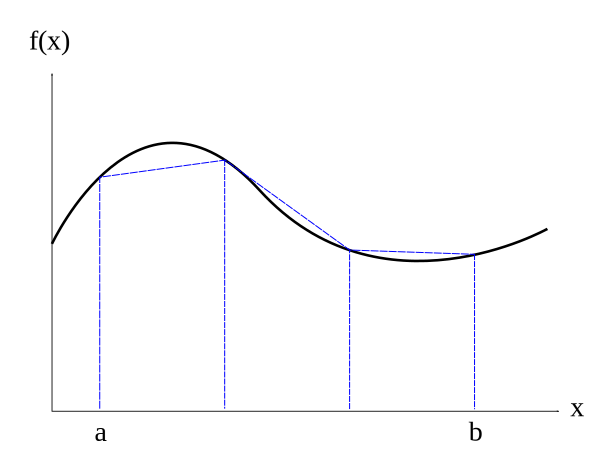
\includegraphics[width=8cm]{integral_diag.pdf}
\caption{Approximating $\int_{x=a}^{b} f(x)$ by summing the area of three trapezoids.
\label{trapezoidfig}}
\end{figure}

We now consider the problem of computing definite integrals
using the trapezoid method. The algorithm is naturally data parallel, and is a common
introductory example in parallel programming tutorials. Our presentation is inspired by
Pacheco's textbook on MPI~\cite{Pacheco}.

We can approximate integrals by summing the area of a consecutive
trapezoids lying under a function within a given interval, as illustrated in
Figure~\ref{trapezoidfig}. A single trapezoid spanning the interval
$[x_0,x_1]$ has area:
\begin{equation*}
\frac{(x_1 - x_0)(f(x_0) + f(x_1))}{2}
\end{equation*}
Extending this to $n$ equally spaced sub-intervals $[x_0,x_1,\ldots,x_n]$ we arrive at the formula:
\begin{equation*}
\begin{split}
\int_{x=a}^{b} f(x)\ \approx\ &\ \frac{h}{2} \sum_{i=1}^n f(x_{i-1}) + f(x_i) \\[3mm]
                     =\  &\ h \left(\frac{f(x_0) + f(x_n)}{2} + f(x_1) + \ldots + f(x_{n-1})\right) \\[3mm]
                     &\ x_0 = a,\ x_n = b,\ h = (b - a)/n\\
                     &\ \forall i \in \{0 \ldots n-1\},\ x_{i+1} - x_{i} = h
\end{split}
\end{equation*}
Listing \ref{Trapezoid} provides a sequential implementation of the trapezoid method in Haskell, with
the integrated function defined to be
$f(x) = sin(x)$.

% ./code/Trapezoid.hs
\begin{listing}
\begin{Verbatim}
module Trapezoid (trapezoid, f) where

trapezoid :: (Double -> Double)  -- Function to integrate
             -> Double -> Double -- integration bounds
             -> Int              -- number of trapezoids
             -> Double           -- width of a trapezoid
             -> Double
trapezoid f a b n h =
   h * (endPoints + internals)
   where
   endPoints = (f a + f b) / 2.0
   internals = worker 0 (a + h) 0.0
   worker :: Int -> Double -> Double -> Double
   worker count x acc
      | count >= n - 1 = acc
      | otherwise = worker (count + 1) (x + h) (acc + f x)

f :: Double -> Double
f = sin
\end{Verbatim}
\caption{Calculating definite integrals using the trapezoid method. \label{Trapezoid}}
\end{listing}
There are undoubtedly more elegant ways to sum the internal points of a trapezoid
than our |worker| function, but we found that GHC produces better compiled code
in this case when given an explicit loop.

% Commented out by Bernie.
%\ezy{Informational note: Sadface! One of my personal research interests
%is making the ``elegant way'' produce code, so I'd personally be
%interested in the version of the function you tried which didn't work so
%well.}

Listing \ref{single-threaded} provides a |main| function which takes
\verb|a|, \verb|b| and \verb|n| from the command line, calls |trapezoid| to compute the integral, and prints
the result.\footnote{Normally, we would check the program inputs for correctness, but in
the interests of saving space, we have elided such checks in the program examples in this article.}
Later on we will provide alternative |main| functions which will parallelize the program
without requiring any changes to |trapezoid| or |f|.

% ./code/single-threaded.hs
\begin{listing}
\begin{Verbatim}
module Main where

import System (getArgs)
import Trapezoid

main :: IO ()
main = do
  aStr:bStr:nStr:_ <- getArgs
  let [a,b] = map read [aStr,bStr]
      n = read nStr
      h = (b - a) / fromIntegral n
      integral = trapezoid f a b n h
  print integral 
\end{Verbatim}
\caption{Sequential program for calculating definite integrals. \label{single-threaded}}
\end{listing}

\section{Parallelization of the trapezoid method on a single machine}

The trapezoid method is a classic data-parallel problem because
the computations on each sub-interval can be computed independently.
For an interval $[a,b]$, $n$ sub-intervals, and $p$ processors, we can parallelize
the algorithm using a simple chunking scheme like so:
\begin{enumerate}
   \item The master processor splits the sub-intervals into chunks of size $s = n/p$ (assuming $n \ge p$).
   \item In parallel, each processor $p_i$ computes the definite integral on the sub-interval 
         $[a_i, b_i]$, where $h = (b - a)/n$, $a_i = a + i \times s \times h$ and
         $b_i = a_i + s \times h$.
   \item The master processor collects the results for each chunk and sums them up.
\end{enumerate}

%./code/multi-threaded.hs
\begin{listing}
\begin{Verbatim}
module Main where

import GHC.Conc
import Control.Parallel.Strategies

import System (getArgs)
import Trapezoid

main :: IO ()
main = do
  let numThreads = numCapabilities
  aStr:bStr:nStr:_ <- getArgs
  let [a,b] = map read [aStr,bStr]
      n = read nStr
      h = (b - a) / fromIntegral n
      localN = n `div` fromIntegral numThreads
      chunks = parMap rseq (\threadNo ->
         let localA = a + fromIntegral (threadNo * localN) * h
             localB = localA + fromIntegral localN * h
             in trapezoid f localA localB localN h) [0..numThreads-1]
  print (sum chunks)
\end{Verbatim}
\caption{Multi-threaded parallel program for calculating definite integrals using the trapezoid method. \label{multi-threaded}}
\end{listing}

Listing~\ref{multi-threaded} shows that it is quite easy to use threads to
parallelize the trapezoid program, thanks to the convenient |parMap| combinator provided by the
parallel strategies library~\cite{parallel_library}.

\section{Parallelization on multiple machines using MPI}

\subsection{Point-to-point communications}

We can use the same chunking approach to parallelize the program
using MPI, whereby the workload is divided over many
independent processes, each with its own private address space.
One of the processes is designated to be the master,
which, in addition to computing its own chunk of the problem, is also responsible for
collecting the results from the other processes and combining them into the final answer.
On a distributed-memory system we can spread the MPI processes over
multiple networked computers (normally one process per core), and thus
scale the parallelization well beyond the number of cores on a single machine.

In multi-threaded programs each parallel task is identified by a simple
numeric index, whereas
MPI uses a two-level numbering scheme.
The first level indicates a group of processes called a communicator;
the second level is the rank of an individual process within such a group.
Each process can participate in an arbitrary number of communicators,
which can be created and destroyed at run time. By default, all
processes are members of the single pre-defined communicator
called |commWorld|.

% Commented out by Bernie.
%\ezy{If a process is identified by a number indicating what communicator
%it is in, how can it participate in arbitrarily many communicators?
%This is not obvious to me.}

Listing \ref{mpi-p2p} shows how to parallelize our program using
two point-to-point communication functions:
\begin{Verbatim}
   send :: Serialize msg => Comm -> Rank -> Tag -> msg -> IO ()
   recv :: Serialize msg => Comm -> Rank -> Tag -> IO (msg, Status)
\end{Verbatim}
The first three arguments of both functions are of the same type.
The first argument is an abstract data
type representing a communicator. In our example program we use
the default |commWorld| for all messaging. The second argument
specifies a process rank. In the case of |send|, it indicates
the identity of receiver, whereas conversely, in the case
of |recv|, it indicates the identity of the sender.
The third argument is a tag which is useful for distinguishing
different messages sent between the same processes.
We do not need this feature in our program, so we have chosen
to make it the dummy value |unitTag|, which is a synonym for |()|.
% Commented out by Bernie.
%\ezy{Technical note: I'm personally a little concerned about the
%lack of type safety of our tags\ldots  the intent is that a Tag
%is only converted to one type in any single program?  Note: I had to
%look at the source to figure out what was going on here.  Perhaps
%mention less.}
However, in general, tags can be any enumerable type.
The fourth argument of |send|, and the first component in
the result of |recv|, is the message itself, which,
in the simple interface of Haskell-MPI, can be any
data type which is an instance of the |Serialize| type class
from the cereal library~\cite{cereal}. Both functions return
an |IO| action as their result; the |send| action yields
unit, and the |recv| action yields a tuple containing
the received message and a status indicator.
By default any errors in
the MPI functions will cause the program to abort, but, by
setting an appropriate error handler, you can
change this behavior so that exceptions are raised instead.

It should be noted that |send| and |recv| are synchronous,
which means that the calling process will block until the message has been
successfully delivered. Non-blocking variants are also available which
return immediately, allowing the processes to do other work while
the message is in transit. A non-blocking receiver must poll for
completion of the message before using its value.

% Commented out by Bernie.
%\ezy{Is this blocking in the Haskell thread sense, or in an
%operating system thread sense?}

Besides point-to-point messaging, MPI
provides one-to-many, many-to-one and many-to-many communication
primitives, capturing the majority of the typical real-world communication
scenarios.

%./code/mpi-p2p.hs
\begin{listing}
\begin{Verbatim}
module Main where

import Control.Parallel.MPI.Simple
import System (getArgs)
import Trapezoid

main :: IO ()
main = mpi $ do
  numRanks <- commSize commWorld
  rank <- commRank commWorld
  let master = 0 :: Rank

  aStr:bStr:nStr:_ <- getArgs
  let [a,b] = map read [aStr,bStr]
      n = read nStr
      h = (b - a) / fromIntegral n
      localN = n `div` fromIntegral numRanks
      localA = a + fromIntegral rank * fromIntegral localN * h
      localB = localA + fromIntegral localN * h
      integral = trapezoid f localA localB localN h
  if rank == master then do
    rest <- sequence [ recv' commWorld (toRank proc) unitTag
                     | proc <- [1..numRanks-1] ]
    print (integral + sum rest)
    else send commWorld master unitTag integral
  where
    recv' comm rank tag = do
      (msg, status) <- recv comm rank tag
      return msg
\end{Verbatim}
\caption{Multi-node parallel program for calculating definite
  integrals, using point-to-point communication. \label{mpi-p2p}}
\end{listing}

In addition to |send| and |recv| the program also calls three other MPI functions:
\begin{Verbatim}
   mpi :: IO () -> IO ()
   commSize :: Comm -> IO Int
   commRank :: Comm -> IO Rank
\end{Verbatim}
The first function takes an |IO| action as input (something which presumably
uses other MPI features) and runs that action within an initialized MPI
environment, before finalizing the environment at the end. The other
functions allow a process to query the total number of processes in a
communicator and the identity of the process within a communicator.

It might seem strange at first that the processes do not exchange any
messages to determine how to divide up the work.
This is unnecessary in our example because all of the important
local information for each process can be deduced from its rank and
the command line arguments, so no additional communication is required.
In other more complex programs it is common to begin the program with
an initialization phase, in which the master sends the configuration
values of the computation to the other processes.

Another surprising aspect of our example is that every MPI process
runs the same executable program, following the so-called
Single Program Multiple Data (SPMD) style. MPI also allows
the Multiple Program Multiple Data (MPMD) style, where
different executables can be run by different processes ---
you can even mix programs written in different languages.
However, the SPMD
style is more common because it reduces development and deployment efforts.
In the SPMD style you typically see blocks of code which are
conditionally executed depending on the value of a the process rank.
In our example, all processes call the |trapezoid| function, but
only the master process calls |recv| and |print|, while
all processes except for the master call |send|.
% Commented out by Bernie.
%If you use MPI in a less-safe language, such as C, care must
%be taken to avoid allocations/computations in processes that would not
%actually use the corresponding data and to avoid using
%uninitialized data. \ezy{Wordy: the point is that we need
%to manage memory in C, right?} Haskell, with its lazy evaluation and automatic
%memory management, makes it much easier to avoid such problems. \ezy{I'm not sure
%lazy evaluation helps for this particular purpose...}
%Pure computations are simply not executed in processes that do not use their
%value, without requiring any explicit housekeeping code.

\subsection{Many-to-one communications}

The use of the point-to-point communications in the previous section
is workable but clumsy. Thankfully, this pattern of many-to-one
% Commented out by Bernie.
%\ezy{(You never
%established that the previous code did have a many-to-one communication pattern!)}
communication is sufficiently common that MPI provides a
convenient way to do it collectively:
\begin{Verbatim}
   gatherSend :: Serialize msg => Comm -> Rank -> msg -> IO ()
   gatherRecv :: Serialize msg => Comm -> Rank -> msg -> IO [msg]
\end{Verbatim}
In this scenario the master process performs a
|gatherRecv| while the others perform a |gatherSend|.
The result of |gatherRecv| is an |IO| action that yields all
the messages from each process in rank order. Note that
the receiver also sends a message to itself, which appears in
the first position of the output list.\footnote{It might seem
strange that the receiver mentions its own rank and passes a message to itself.
These oddities are required by a feature of
MPI called intercommunicators. We do not discuss them in this
article, but an interested reader can consult the MPI report
for more details~\cite{mpi-report}.} The collective communications
cannot be overlapping, so there is no need for a tag argument to
distinguish between them.\footnote{See Chapter 5 of the MPI report~\cite{mpi-report}.}
%\ezy{Consider briefly mentioning data backing
%this claim, maybe a cite is enough.}

%./code/mpi-gather.hs
\begin{listing}
\begin{Verbatim}
module Main where

import Control.Parallel.MPI.Simple
import System (getArgs)
import Trapezoid

main :: IO ()
main = mpi $ do
  numRanks <- commSize commWorld
  rank <- commRank commWorld
  let master = 0 :: Rank

  aStr:bStr:nStr:_ <- getArgs
  let [a,b] = map read [aStr,bStr]
      n = read nStr
      h = (b - a) / fromIntegral n
      localN = n `div` fromIntegral numRanks
      localA = a + fromIntegral rank * fromIntegral localN * h
      localB = localA + fromIntegral localN * h
      integral = trapezoid f localA localB localN h
  if rank == 0
     then print . sum =<< gatherRecv commWorld master integral
     else gatherSend commWorld master integral
\end{Verbatim}
\caption{Multi-node parallel program for calculating definite
  integrals, using many-to-one communication. \label{mpi-gather}}
\end{listing}

As you can see in Listing \ref{mpi-gather},
the use of collective communications
leads to a much more succinct implementation of the program.
However, this is not their only virtue. An MPI implementation
can take advantage of the underlying network hardware to optimize
the collective operations, providing significant performance
gains over point-to-point versions.

\section{Performance results}

We now consider a small benchmark test to get a feeling for how well Haskell-MPI performs
in practice. For comparison we ran the same test on three alternative implementations
of the same program: the baseline sequential program,
the multi-threaded Haskell version, and a C version which also uses MPI.

All performance tests were executed on an IBM iDataplex cluster,
featuring 2.66GHz Intel Nehalem processors, with 8 cores and
24GB of RAM per node, running Red Hat Enterprise Linux 5, connected
to a 40 Gb/s InfiniBand network. We used the following software
versions to build the programs:
\begin{enumerate}
   \item GHC 7.0.3, with optimization flags |-O2|.
   \item GCC 4.4.4, with optimization flags |-O2|.
   \item Open MPI 1.4.2.
\end{enumerate}

The benchmark test case computes the definite integral of Sine
on the interval $[0,1000\pi]$, using $10^9$ trapezoids.
We had to choose a very large number of trapezoids to
make it worth parallelizing this toy example at all.

%\ezy{In the figure below, it took me a while to figure out what was
%meant by ``scaling''.  Maybe this is just because I haven't looked
%at enough multicore scaling papers, but it is an odd little metric
%that represents the relationship between two rows in the table, not
%just one.}

%\ezy{I'm confused why C manages to scale more than two times when two
%cores are used. Any guesses why?}

\begin{figure}
\begin{minipage}[t]{0.5\linewidth}\centering
Haskell \\[3mm]
\begin{tabular}{llll}
method & cores & time(s) & scaling \\ \hline
MPI & 1   & 54.364  & -- \\
MPI & 2   & 26.821  & 2.0 \\
MPI & 4   & 12.022  & 2.2 \\
MPI & 8   & 6.142   & 2.0 \\
MPI & 16  & 4.975   & 1.2 \\
MPI & 32  & 3.952   & 1.3 \\
MPI & 64  & 3.291   & 1.2 \\
MPI & 128 & 3.141   & 1.0 \\
MPI & 256 & 3.674   & 0.9 \vspace{0.5em} \\
sequential & 1     & 54.301  & --  \vspace{0.5em} \\
threads & 1    & 48.866  & -- \\
threads & 2    & 24.118  & 2.0 \\
threads & 4    & 12.080  & 2.0 \\
threads & 8    & 6.014  &  2.0 \\
\end{tabular}
\end{minipage}
\begin{minipage}[t]{0.5\linewidth}
\centering
C \\[3mm]
\begin{tabular}{llll}
method & cores & time(s) & scaling \\ \hline
MPI & 1      & 53.570  & -- \\
MPI & 2      & 23.664  & 2.3 \\
MPI & 4      & 12.500  & 1.9 \\
MPI & 8      &  6.656  & 1.9 \\
MPI & 16     &  4.142  & 1.6 \\
MPI & 32     &  3.360  & 1.2 \\
MPI & 64     &  3.037  & 1.1 \\
MPI & 128    &  2.861  & 1.1 \\
MPI & 256    &  2.934  & 1.0 \\
\end{tabular}
\end{minipage}
\vspace{3mm}
\caption{Performance figures for sequential, threaded and MPI versions of the trapezoid program,
when integrating Sine on the interval $[0,1000 \pi]$ using $10^9$ trapezoids. \label{TiminigTable}}
\end{figure}

\begin{figure}
\centering
\includegraphics{performance.pdf}
\vspace{3mm}
\caption{Performance comparison of sequential, threaded and MPI versions of the trapezoid program.
\label{PerformanceGraph}}
\end{figure}

Figure~\ref{TiminigTable} shows the raw benchmark results taken by averaging three
simultaneous runs of the same computation. Figure~\ref{PerformanceGraph}
plots the results on a graph. The tests illustrate that we get strong scaling
for all parallel implementations up to 8 cores. The performance improvement of
the MPI implementations is fairly similar with
a slight edge to the C version. Scaling tends to decline around
the 16 core mark, although small improvements in overall performance are made up to
128 cores, but both programs begin to slow down at 256 cores.
The threaded implementation stops at 8 cores because that is the maximum available
on a single node in our test machine.
Given more cores in a single node we might expect the threaded version to
show similar improvements to the MPI versions. Having said that, the limitation
of the threaded version to a single shared-memory instance will ultimately be
a barrier to very large-scale parallelism on current hardware.
However, there is nothing to stop you from using threads within an MPI application.

Obviously, we should not to pay too much heed to one toy benchmark.
We would need a much bigger problem to show strong scaling beyond a dozen or so cores,
and a truly gigantic problem to scale to the size of a machine such as LLNL's
upcoming Sequoia!

\subsection{The Simple and Fast interfaces of Haskell-MPI}

One of the biggest limitations of our test case is that we are only sending trivially
small messages between processes (individual double precision floating point numbers).
%\ezy{But maybe sending lots of small messages imposes its own overhead.  Does
%this particular example need to send a length, for example?}
For larger messages the simple interface to Haskell-MPI imposes additional
performance costs due to the need to make a copy of the data for serialization. %\ezy{Awkward.}
Furthermore, in many cases, each message sent is preceded implicitly by another
message carrying size information about the serialized data stream.
For this reason Haskell-MPI provides an alternative ``fast'' interface which works
on data types that have a contiguous in-memory representation, thus avoiding
the need for serialization. \verb|ByteString|s, unboxed arrays, and
instances of the \verb|Storable| type class can all be handled this way. The fast interface is more
cumbersome to use, but it is a necessary evil for programs with large message sizes
and tight performance constraints.

\section{Conclusion}

Haskell-MPI provides a pragmatic way for Haskell programmers to write high performance programs in
their favorite language today. The current version of the library covers the most commonly used parts of
the MPI standard, although there are still several missing features, the most significant of which is
parallel I/O. We plan to include more parts of the standard over time, with emphasis on those
which are requested by users.

As you can see from the examples presented in this article, Haskell-MPI
does not provide a particularly functional interface to users -- most of the provided functions return
|IO| results, and there is no satisfying way to send functions as messages. This reflects the
modest ambitions of the project, but we may investigate more idiomatic APIs in future work.

\section{Acknowledgments}

Dmitry's work on Haskell-MPI was funded by Microsoft Research and the Well-Typed LLP partnership as a part of the Parallel Haskell project.

All the performance tests for this article were executed on one of the x86 clusters at the
Victorian Life Sciences Computation Initiative (VLSCI), in Melbourne, Australia~\cite{VLSCI}.
We would like to thank the VLSCI for
generously donating time on their computers for our work.

Michael Weber and Hal Daum\'{e} III provided an earlier Haskell binding to MPI called hMPI. Their work
provided much inspiration for Haskell-MPI, especially in the early stages of development.

We would also like to thank Duncan Coutts, Ben Horsfall, Chris Samuel, Lee Naish, John Wagner, Edward Yang and Brent Yorgey for providing
comments on earlier drafts of this article.

The full text of this article and all accompanying code is available on GitHub under the BSD3 license (see \cite{article}).

\section{Appendix A: Installation and configuration}
\label{appendix-A}
In order to use Haskell-MPI you need to have one of the
MPI libraries installed on your computer. If you don't already have one installed, then 
Open MPI %\ezy{Cite please!} 
is a good choice. We've tested Haskell-MPI with
Open MPI 1.4.2 and 1.4.3 and MPICH 1.2.1 and 1.4, and there is a good chance it
will work with other versions out of the box.

If the MPI libraries and header files are in the search paths of your C
compiler, then Haskell-MPI can be built and installed with the
command:\footnote{MPICH v1.4 requires extra argument \verb|-fmpich14|}
\begin{Verbatim}
   cabal install haskell-mpi
\end{Verbatim}
Otherwise, the paths to the include
files and libraries need to be specified manually:
\begin{Verbatim}
   cabal install haskell-mpi \
     --extra-include-dirs=/usr/include/mpi \
     --extra-lib-dirs=/usr/lib/mpi
\end{Verbatim}

If you are building the package with an MPI implementation other than
Open MPI or MPICH, it is recommended to pass \verb|-ftest| to
\verb|cabal install|, running the test-suite to verify that the bindings
perform as expected. If you have problems configuring MPI, take a
look at the useful hints in the Haddock documentation for the module \verb|Testsuite|.

\bibliography{haskell-mpi}
\end{document}
